\documentclass[aspectratio=43]{beamer}
\usepackage[latin1]{inputenc}
\usepackage{amsmath}
\usepackage{amsfonts}
\usepackage{amssymb}
\usepackage{makeidx}
\usepackage{graphicx}
\usepackage{array}

% Customization
\mode<presentation>{
\usetheme{CambridgeUS}
\usecolortheme{dolphin}
\setbeamertemplate{navigation symbols}{}
}

% Define colors
\definecolor{darkgreen}{rgb}{0.0, 0.5, 0.13}
\definecolor{darkblue}{rgb}{0.0, 0.0, 0.55}
\definecolor{darkred}{rgb}{0.55, 0.0, 0.0}

%************************************************************************************************************

% Title and author
\title[QCD and Monte Carlo]{QCD and Monte Carlo}
\author{\textbf {Jes\'us Urtasun Elizari}}
\date{Milan, February 2021}

\begin{document}

% Front slide
\begin{frame}
	
	%\maketitle
	\vspace{1.0 cm}
	
	\center{\color{blue}QCD and Monte Carlo event generators}
	
	\vspace{0.25 cm}
	\center{Monte Carlo course seminar - Milan, February 2021}

	\begin{figure}
		\minipage{1\textwidth}
		
\includegraphics[width = 3.0 cm]{plots/logo_unimi.png}
		\hfill
		
\includegraphics[width = 3.0 cm]{plots/logo_infn.png}
		\hfill
		
\includegraphics[width = 3.0 cm]{plots/logo_erc.png}
		\endminipage
	\end{figure}

	\vspace{1.0 cm}

\end{frame}

% Introduction
\begin{frame}

	\frametitle{Outline}
	
	\begin{enumerate}
		\item {\color{blue}Hadron collisions and strong interactions}
		\begin{itemize}
			\item Hadron collisions and strong interactions
			\item Renormalization group
			\item IR divergences
		\end{itemize}
		\item {\color{blue}MC and Parton Showers}
		\begin{itemize}
			\item Factorization theorem
			\item Final state radiation
			\item Initial state radiation
		\end{itemize}
		\item {\color{blue}Hadronization: some basics}
	\end{enumerate}
	
\end{frame}

% Strong interactions I
\begin{frame}

	\frametitle{Strong interactions}
	\framesubtitle{QCD from $e^{+}e^{-}$ annihilation}

	Quantum Chromodynamics (QCD) $\rightarrow$ theory describing the interaction between quarks and gluons (strong interactions)
	\begin{figure}
		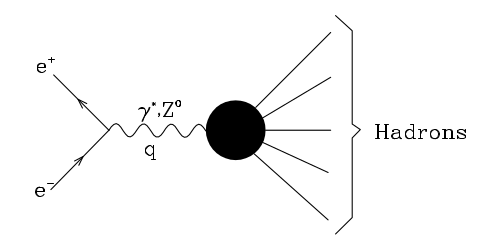
\includegraphics[width = 5 cm]{plots/ee_hadrons.png}
	\end{figure}
 
	QCD arises already from $e^{+}e^{-}$ annihilation $\rightarrow R_{0}$ ratio

	\begin{columns}
	
		\column{0.5\textwidth}
	
		\begin{figure}
			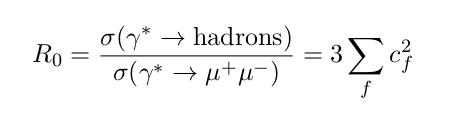
\includegraphics[width = 6 cm]{plots/eq_R0.png}
		\end{figure}
	
		\column{0.5\textwidth}
	
		\begin{enumerate}
			\item \footnotesize Color factor (3 color for each quark)
			\item \footnotesize Sum over charges of different flavors
			\item \footnotesize Threshold and higher order corrections
		\end{enumerate}	

	\end{columns}

\end{frame}

% Strong interactions II
\begin{frame}
	
	\frametitle{Strong interactions}
	\framesubtitle{QCD from $e^{+}e^{-}$ annihilation}
	
	Questions for a field theory
	
	\vspace{0.3cm}
	
	\begin{enumerate}
		\item Can we go to arbitrarily large energies? $\rightarrow$ divergences arise, renormalization / factorization needed
		\item Can we compute $R_{0}$ for every process? $\rightarrow$ IR observables
	\end{enumerate}	

\end{frame}

% Renormalization group I
\begin{frame}

	\frametitle{Strong interactions}
	\framesubtitle{Renormalization group}
	
	\begin{itemize}
		\item Running coupling given by Renormalization Group Equation (RGE)
		\begin{equation}
			{\color{blue}\mu\frac{d\alpha_{s}(\mu)}{d\mu} = \beta(\alpha_{s}(\mu)) = -\sum_{n = 0}^{\infty} \beta_{n} \Big( \frac{\alpha_{s}}{\pi} \Big)^{n + 1}} \nonumber
		\end{equation}
		\item Coupling {\color{blue}$\alpha_{s}$} evolves with scale {\color{blue}$\mu$} as given by RGE $\rightarrow$ LO behavior driven by $\beta_{0}$
		\item $\beta_{0}^{\textrm{QCD}} > 0 \implies$ weakly coupled at large energies, asymptotic freedom
		\item $\beta_{0}^{\textrm{QED}} < 0 \implies$ strongly coupled at large energies, UV divergent!	
	\end{itemize}

\end{frame}

% Renormalization group II
\begin{frame}

	\frametitle{Strong interactions}
	\framesubtitle{Renormalization group}

	\begin{columns}	
	
		\column{0.5\textwidth}
		
		\begin{figure}
			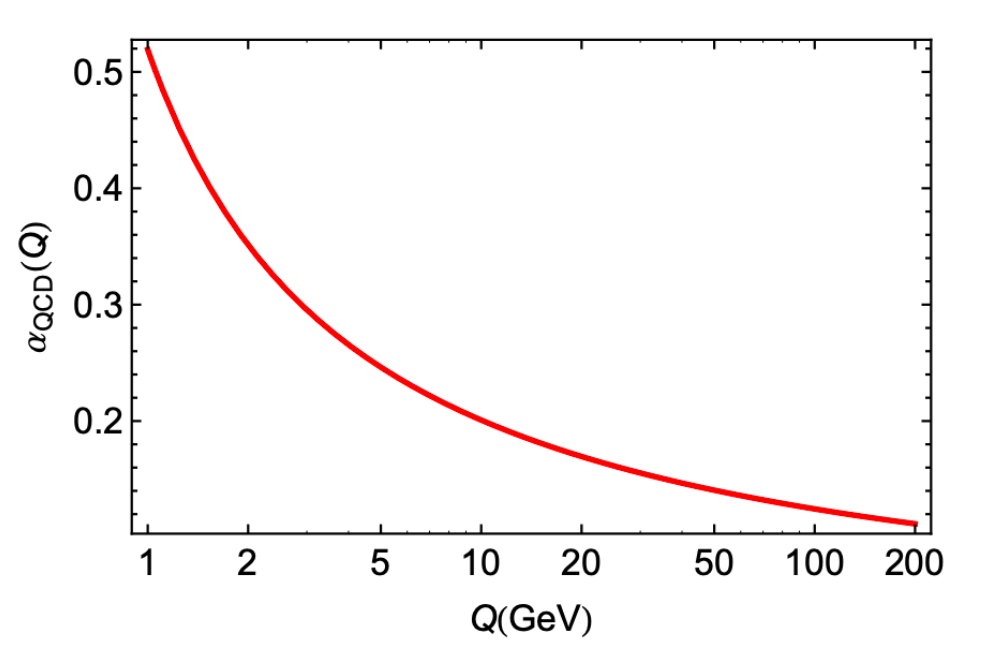
\includegraphics[width = 5 cm]{plots/qcd_coupling.png}
		\end{figure}

		\column{0.5\textwidth}
	
		\begin{itemize}
			\item \footnotesize Running coupling given by Renormalization Group Equation (RGE)
			\begin{equation}
				\alpha_{s}(\mu) = \frac{1}{b_{0} \log\big( \frac{\mu^{2}}{\Lambda_{s}^{2}}\big)} \nonumber
			\end{equation}
			\item \footnotesize $\beta_{0}$
			\item \footnotesize $\Lambda_{s}$
		\end{itemize}

	\end{columns}
	
	\vspace{1cm}
	\center QCD is weakly coupled for $\mu >> \Lambda_{s} \longrightarrow$ asymptotically free
	\center \color{red} Perturbative Quantum Chromodynamics (pQCD)

\end{frame}

% Factorization theoren
\begin{frame}

	\frametitle{Factorization theorem}
	\framesubtitle{QCD factorization}
	
	\center \footnotesize LHC processes $H_{1} + H_{2} \rightarrow \textrm{F}$
	
	\begin{figure}
		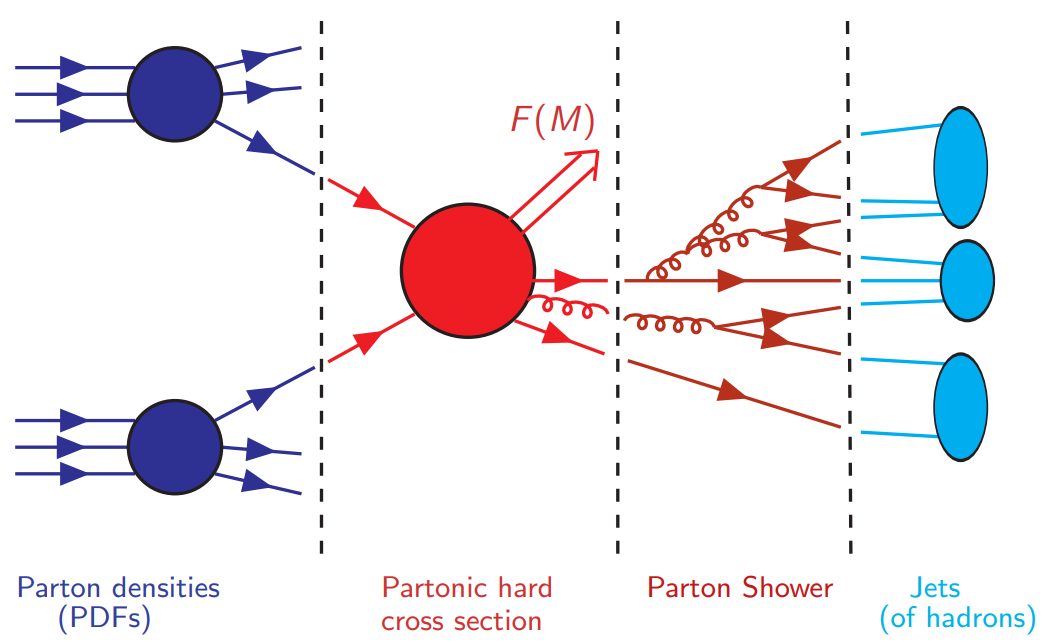
\includegraphics[width = 7 cm]{plots/factorization_1.png}
	\end{figure}
	
	\footnotesize {Separate process {\color{blue}PDFs} and {\color{red} partonic (hard) interaction}	
	\begin{equation}
		\sigma^{\textrm{F}}(p_{1}, p_{2}) =
		\int_{0}^{1} dx_{1} dx_{2} \; {\color{blue} f_{\alpha}(x_{1}, \mu_{F}^{2}) \ast f_{\beta}(x_{2}, \mu_{F}^{2})}
		\; \ast \;  
		{\color{red}\hat{\sigma}^{\textrm{F}}_{\alpha \beta}(x_{1}p_{1}, x_{2}p_{2}, \alpha_{s}(\mu_{R}^{2}), \mu_{F}^{2})} \nonumber
	\end{equation}}
		
\end{frame}

% Parton showers I
\begin{frame}

	\frametitle{Parton showers}
	\framesubtitle{MC Parton showers}
	
	\footnotesize Partons in the initial and final state emit radiation. State Radiation (ISR) and Final State Radiation (FSR)
	
	\vspace{0.1 cm}
	\center \color{red} Shower Monte Carlo programs (HERWIG, PYTHIA)
	\vspace{0.15 cm}
	
	\begin{itemize} 
		\item Libraries for computing SM and BSM cross sections
		\item Shower algorithms produce the parton shower from final state or initial state partons
		\item Hadronization models, underlying event, decays of unstable hadrons, etc
	\end{itemize}

\end{frame}


% Parton showers II
\begin{frame}

	\frametitle{Parton showers}
	\framesubtitle{Collinear limit}
	
	\begin{itemize} 
		\item An emitted parton is collinear to an incoming or outgoing parton ($\theta$ small)
		\item Measurement not sensitive to such small scales
		\item $\sigma$ dominated by collinear emission $q \rightarrow qg, g \rightarrow gg, g \rightarrow q\bar{q}$
	\end{itemize}
	
	\begin{figure}
		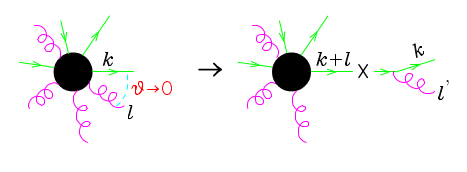
\includegraphics[width = 7 cm]{plots/collinear_factorization.png}
	\end{figure}
	
	Collinear factorization $\longrightarrow$ Factor out tree level amplitude and splitting
	\begin{figure}
		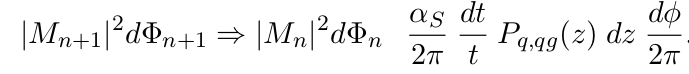
\includegraphics[width = 8 cm]{plots/eq_factorization_theorem.png}
	\end{figure}

\end{frame}

% Parton showers III
\begin{frame}

	\frametitle{Parton showers}
	\framesubtitle{Kinematics of splitting}
	
	\begin{itemize} 
		\item Kinematics of splitting $(t, z, \phi)$
		\begin{itemize}
			\item $t$ has dimensions of energy (virtuality, $p_{\perp}$, angular variable)
			\item $z$ represents the fraction of momentum of radiated parton
			\item $\phi$ represents azimuth of the $k, l$ plane
		\end{itemize}
	
	\vspace{0.5cm}
	
		\item Factorization holds for small angles. Applied recursively
	\end{itemize}
	
	\begin{figure}
		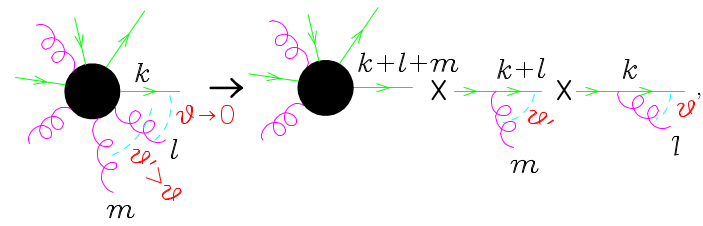
\includegraphics[width = 7 cm]{plots/shower_4.png}
	\end{figure}

\end{frame}

% Parton showers IV
\begin{frame}

	\frametitle{Parton showers}
	\framesubtitle{AP splitting functions}
	
	Altarelli-Parisi splitting functions
	
	\begin{figure}
		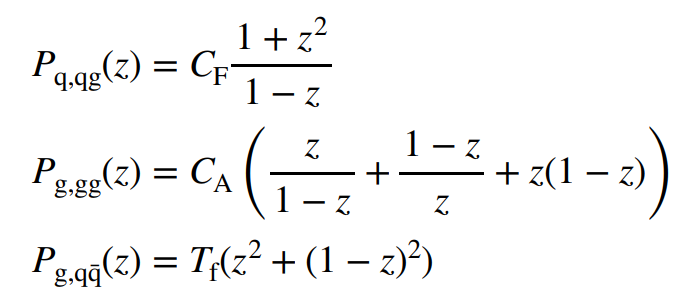
\includegraphics[width = 5 cm]{plots/AP_splitting.png}
	\end{figure}

	We can proceed in an iterative way
	\begin{figure}
		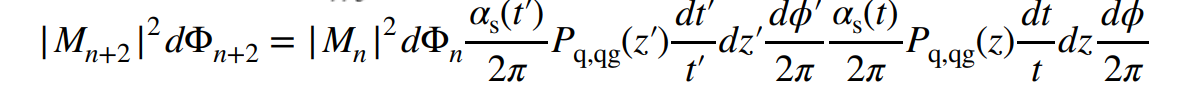
\includegraphics[width = 9 cm]{plots/AP_iteration.png}
	\end{figure}

	\footnotesize Exclusive final state: limit to the most singular terms, in ordered sequence of angles
	\color{red} Collinear approximation $\longrightarrow$ Leading log approximation
	
\end{frame}

% FSR MC I
\begin{frame}

	\frametitle{Final state radiation MC}
	\framesubtitle{General structure}
	
	\footnotesize Approximated description of a hadronic final state. Model a given hard scattering with arbitrary number of enhanced radiations

	\begin{itemize} 
		\item Choose hard interaction with specified Born kinematics.
		\item Consider all possible splittings for each coloured parton.
		\item Assign the variables t, z, $\phi$ at each splitting vertex, t ordered in decreasing way.
		\item At each splitting vertex assign the weight (...)
		\item Each line has a weight known as Sudakov factor (...)
	\end{itemize}

\end{frame}

% FSR II - Formal representation of a shower
\begin{frame}

	\frametitle{Final state radiation MC}
	\framesubtitle{Formal representation of a shower}
	
	Approximated description of a hadronic final state. Model a given hard scattering with arbitrary number of enhanced radiations
	
	\begin{figure}
		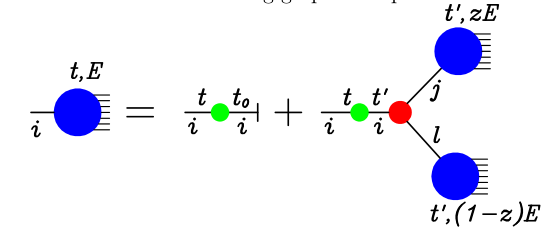
\includegraphics[width = 6 cm]{plots/shower_2.png}
	\end{figure}
		
	Forward evolution equation
	\begin{figure}
		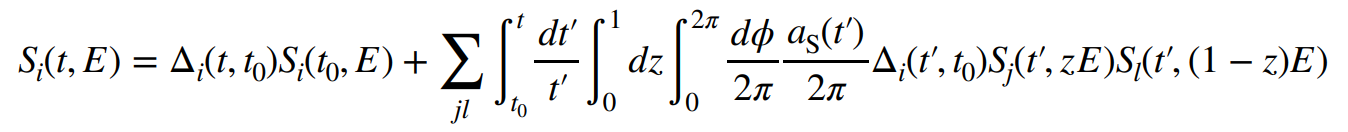
\includegraphics[width = 10 cm]{plots/shower_0.png}
	\end{figure}

\end{frame}

% FSR III - Formal representation of a shower
\begin{frame}

	\frametitle{Final state radiation MC}
	\framesubtitle{Probabilistic interpretation}
	
	\begin{figure}
		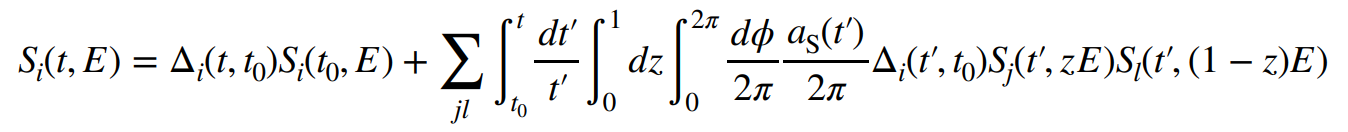
\includegraphics[width = 3 cm]{plots/shower_0.png}
	\end{figure}
	
	\begin{figure}
		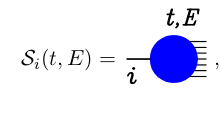
\includegraphics[width = 3 cm]{plots/shower_1.png}
	\end{figure}

	\begin{figure}
		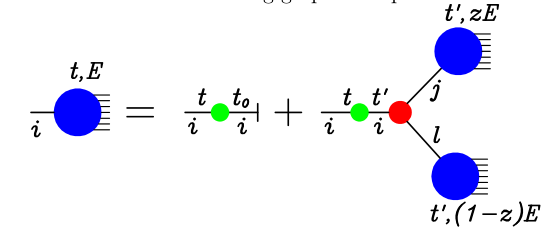
\includegraphics[width = 3 cm]{plots/shower_2.png}
	\end{figure}

	\begin{figure}
		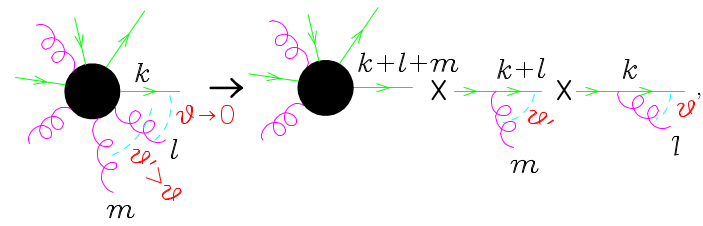
\includegraphics[width = 3 cm]{plots/shower_4.png}
	\end{figure}


\end{frame}

FSR IV - MC programs
\begin{frame}

	\frametitle{Final state radiation MC}
	\framesubtitle{Shower algorithm}
	
	Generate hard process with probability proportional to its parton level cross section. For each final state colored parton:
	\begin{enumerate} 
		\item Set scale $t = Q$, hard scale of the process
		\item Generate random number $0 < r < 1$
		\item Solve $r = \Delta_{i}(t, t')$ for t'
		\item i) if $t' < t_{0}$, no further branching and stop shower
		\item ii) if $t' \geq t_{0}$, one branching into partons $j, l$ with energies $E_{j} = zE_{i}$ and $E_{l} = (1 - z)E_{i}$, z following the $P_{i, jl}(z)$ distribution and $\phi$ uniform in the interval $[0, 2\pi]$ (variables, ...)
		\item For each branched partons set $t = t'$ and start from (2)
	\end{enumerate}

\end{frame}

% ISR MC I
\begin{frame}

	\frametitle{Initial state radiation MC}
	\framesubtitle{General structure}
	
	\begin{figure}
		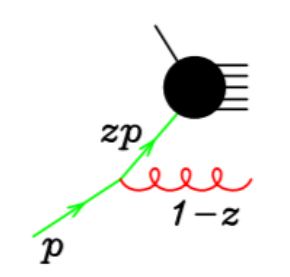
\includegraphics[width = 3 cm]{plots/shower_ISR_0.png}
	\end{figure}
	
	\begin{itemize} 
		\item Lines between $t_{1}$ and $t_{2}$ (consecutive radiations) are spacelike {\color{blue}(*)}
		\item Difference in Sudakov factors and Splitting functions start at NLO
	\end{itemize}
	
	\begin{figure}
		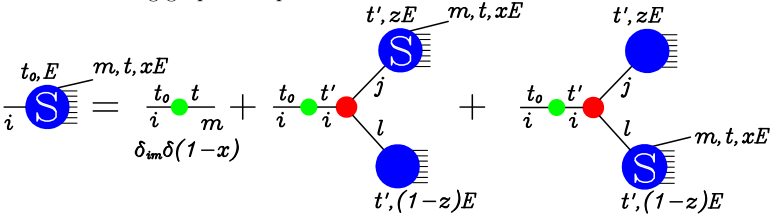
\includegraphics[width = 10 cm]{plots/shower_ISR_3.png}
	\end{figure}

\end{frame}

% ISR MC II
\begin{frame}
	
	\frametitle{Initial state radiation MC}
	\framesubtitle{Formal representation}
	
	\begin{figure}
		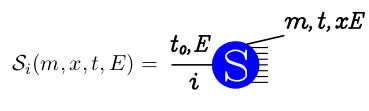
\includegraphics[width = 3 cm]{plots/shower_ISR_2.png}
	\end{figure}
	
	\begin{itemize} 
		\item Lines between $t_{1}$ and $t_{2}$ (consecutive radiations) are spacelike {\color{blue}(*)}
		\item Difference in Sudakov factors and Splitting functions start at NLO
	\end{itemize}
	
	Forward evolution equation. Great amount of computation time to generate configurations -> the scattering that we want
	\begin{figure}
		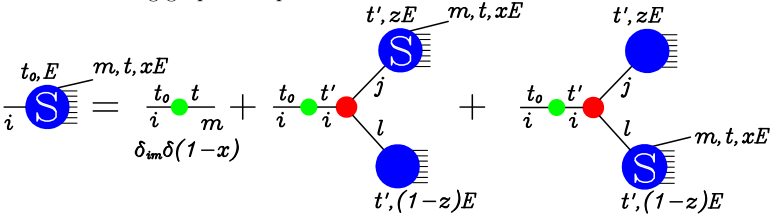
\includegraphics[width = 10 cm]{plots/shower_ISR_3.png}
	\end{figure}

\end{frame}

% ISR MC III
\begin{frame}
	
	\frametitle{Initial state radiation MC}
	\framesubtitle{Formal representation}
	
	\begin{figure}
		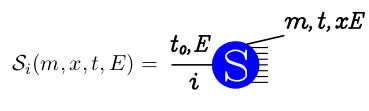
\includegraphics[width = 3 cm]{plots/shower_ISR_2.png}
	\end{figure}
	
	\begin{itemize} 
		\item Lines between $t_{1}$ and $t_{2}$ (consecutive radiations) are spacelike {\color{blue}(*)}
		\item Difference in Sudakov factors and Splitting functions start at NLO
	\end{itemize}
	
	Backward evolution equation
	\begin{figure}
		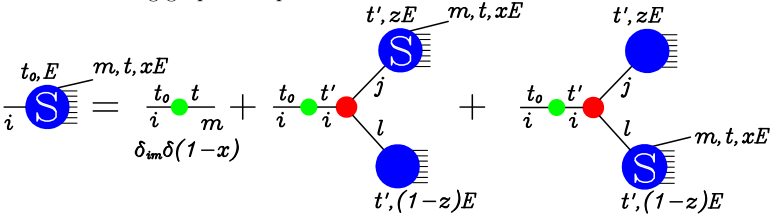
\includegraphics[width = 10 cm]{plots/shower_ISR_3.png}
	\end{figure}

\end{frame}

% ISR MC IV
\begin{frame}

	\frametitle{Initial state radiation MC}
	\framesubtitle{Shower algorithm}
	
	Generate hard process with probability proportional to its parton level cross section. For each final state colored parton:
	\begin{enumerate} 
		\item Set scale $t$ to $Q$, hard scale of the process
		\item Generate random number $0 < r < 1$
		\item Solve (...) for t'
		\item i) if $t' < t_{0}$, no further branching and stop shower
		\item ii) if $t' \geq t_{0}$, one branching into partons $j, l$ with energies $E_{j} = zE_{i}$ and $E_{l} = (1 - z)E_{i}$, z following the $P_{i, jl}(z)$ distribution and $\phi$ uniform in the interval $[0, 2\pi]$
		\item For parton j (...), for parton l generate a timelike parton shower according to the algorithm shown previously
	\end{enumerate}

\end{frame}

% Hadronization I
\begin{frame}
	
	\frametitle{Hadronization}
	\framesubtitle{Basics}

\end{frame}

% Hadronization II
\begin{frame}
	
	\frametitle{Hadronization}
	\framesubtitle{Lund string model}

\end{frame}

% Hadronization III
\begin{frame}
	
	\frametitle{Hadronization}
	\framesubtitle{Clustering models}

\end{frame}









% Shower equation II
\begin{frame}

	\frametitle{Parton showers and MC generators}
	\framesubtitle{Formal representation of a shower}
	 
	 
	 Ensemble of all possible radiations as the sum of no radiation, with radiation and shower from radiated partons
	\begin{figure}
		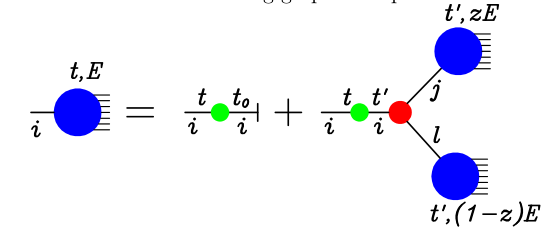
\includegraphics[width = 7 cm]{plots/shower_2.png}
	\end{figure}
	
	\begin{itemize} 
		\item Ansatz for Sudakov $$\Delta_{i}(t, t') = \exp\Bigg\{- \int_{t'}^{t} \frac{dt''}{t''}\int dz \sum_{jl} P_{i, jl}(z) \frac{\alpha_{s}(t')}{2\pi} \Bigg\}$$
		\item Therefore $\partial \Delta(t, t') / \partial t \propto \Delta(t, t') \longrightarrow$ apply shower recursively
	\end{itemize}

\end{frame}

% Shower equation III
\begin{frame}

	\frametitle{Parton showers and MC generators}
	\framesubtitle{Shower algorithm}
	
	Generate hard process with probability proportional to its parton level cross section. For each final state colored parton:
	\begin{enumerate} 
		\item Set scale $t$ to $Q$, hard scale of the process
		\item Generate random number $0 < r < 1$
		\item Solve $r = \Delta_{i}(t, t')$ for t'
		\item i) if $t' < t_{0}$, no further branching and stop shower
		\item ii) if $t' \geq t_{0}$, one branching into partons $j, l$ with energies $E_{j} = zE_{i}$ and $E_{l} = (1 - z)E_{i}$, z following the $P_{i, jl}(z)$ distribution and $\phi$ uniform in the interval $[0, 2\pi]$
		\item For each branched partons set $t = t'$ and start from (2)
	\end{enumerate}

\end{frame}

% Shower equation ISR I
\begin{frame}

	\frametitle{Parton showers and MC generators}
	\framesubtitle{Initial state radiation}
	
	ISR already important in QED $\longrightarrow$ Used to determine the $Z$ peak at LEP
	\begin{figure}
		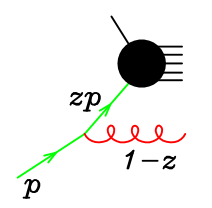
\includegraphics[width = 3 cm]{plots/shower_ISR.png}
	\end{figure}
	
	\begin{itemize}
		\item QCD coupling much larger $\longrightarrow$ QCD ISR even more important
		\item Specially large for small momentum transfer
		\item Same as final state partons \textit{always} manifest as jets, initial state ones \textit{always} lead to ISR
	\end{itemize}
	
\end{frame}

% Shower equation III
\begin{frame}

	\frametitle{Parton showers and MC generators}
	\framesubtitle{Ordering variables}
	
	HERWIG
	\begin{itemize} 
		\item Ordering variable $t = E^{2}\theta^{2}/2$
		\item Order of transverse momentum as "angular ordering"
		\item IR cut-off needed
	\end{itemize}

	PYTHIA
	\begin{itemize} 
		\item There is not angular ordering
		\item More natural kinematics
		\item Unphysical increase of number of partons $\longrightarrow$ solve by imposing veto to branchings that violate angular ordering
	\end{itemize}

\end{frame}

\end{document}